\section{Detection \& Eviction}
\label{sec:detection}

In this section, we describe the main building blocks that constitutes proposed detection mechanism that targets detecting malicious peers in order to restore benign peers satisfaction.
We start by highlighting the general overview on how the detection mechanism flows.
Then, we describe the main differences between detecting a dropping attack behavior and detecting a manipulation/outdated chunks attack behavior, referred to as \textit{drop} attack, \textit{manp} attack for simplicity.
Afterwards, each detection sub-block, as illustrated in Figure~\ref{detection-blocks}, is presented.
The list of variables used throughout the paper is provided in Table \ref{tab:acronyms}.

\begin{table}[ht]
\center
\caption{Acronyms}
\begin{tabular}{|c|l||c|l|}
\hline

\bf{Var.} & \bf{Description}  & \bf{Var.} & \bf{Description} \\\hline\hline
$x$ & no. of malicious peers & $\eta$ & mal. headnodes fraction\\\hline
$MN$ & malicious neighbors & $\sigma$ & satisfaction threshold\\\hline
$H_n$ & list of headnodes & $P_n$ & potential candidates list \\\hline
$\alpha$ & manipulation threshold& $F$ & familiarity of suspect \\\hline
$G$ & suspect guilt value & $\kappa$ & dropping det. allowed\\\hline
$NL$ & neighbor list & $BM$ & buffer map\\\hline
\end{tabular}
\label{tab:acronyms}
\end{table}

\subsection{Mechanism Overview}
Here we describe an overall view for the flow of the detection mechanism before every process is detailed through the rest of the section.
Once a detection condition is triggered by a peer $b$, it sends a detection request to all peers that exist in its neighbor list.
Afterwards, for each peer who receives a request, prepares a reply according to the request ID, i.e., a \textit{drop} or a \textit{manp} request.
Once $b$ collects all the replies, it decides according to the proposed detection from the  in the replies to whether to fire a complaint to the source or not.
$b$ sends the complaint on behalf of the participating peers in the detection request. 
Finally, if $b$ sends a complaint to the source, the source decides about its content and replies back to $b$. In turn, $b$ forwards the source reply to the other participants in the complaint.

\subsection{Drop vs. Manp Detection}

On one hand, when $m$ conducts a drop attack on $b$, $b$ is not capable of detecting any malicious behavior.
Specifically, in a drop attack, $m$ never sends the actual $BM$ that represents the chunks it currently possesses, i.e., $m$ is only requesting chunks it already has.

On the other hand, in a manipulation or outdated chunks behavior, $m$ is eventually suspected as malicious since $b$ already expects the requested chunk from $m$.
Note that a peer might be overloaded due to a tight upload bandwidth or serving a lot of peers and thus, not able to serve all the requests.
Accordingly, the detection mechanism should differentiate between a malicious manipulating peer and an overloaded peer, which is discussed in Section~\ref{Detection-Trigger}.
To that end, through the rest of the section, we describe how the detection mechanism handles both cases: Drop and Manp detection.

\begin{figure}
 \centering
 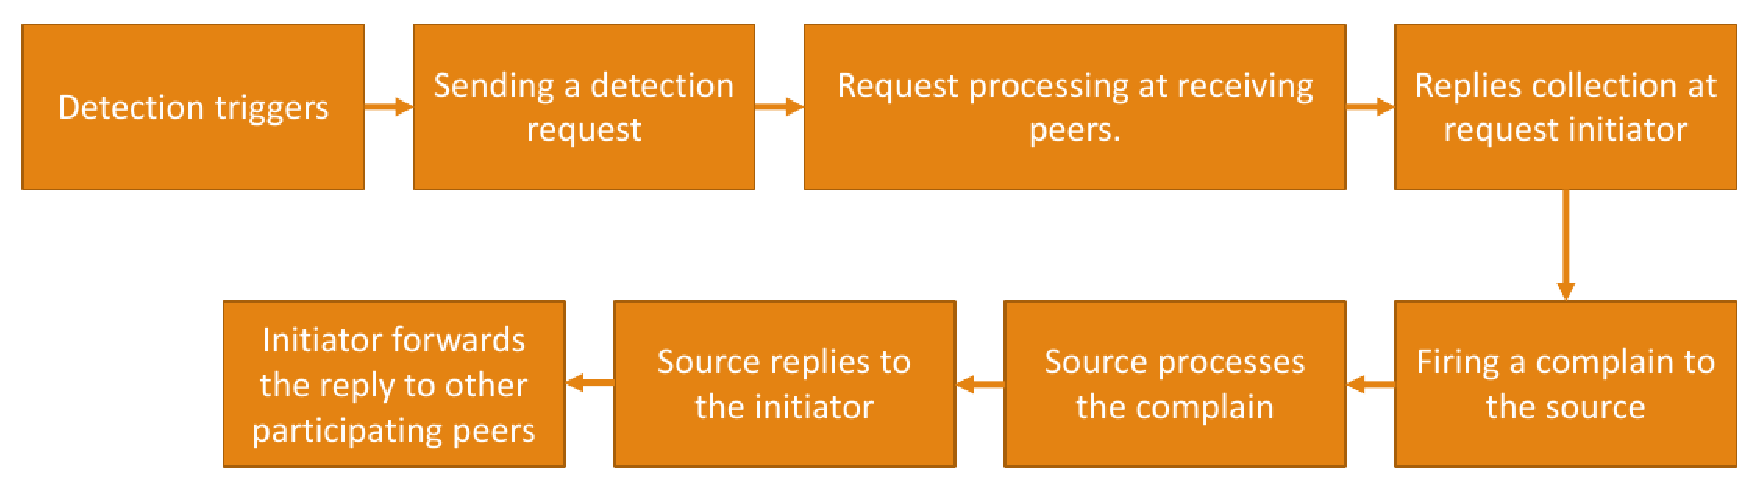
\includegraphics[width=8cm,height=3cm]{./Figures/detection-blocks.eps}
  \caption{Detection mechanism main blocks}
\label{detection-blocks} 
\end{figure}

\subsection{Detection Trigger}
\label{Detection-Trigger}
Here we describe how a peer decides on sending a detection request for both attack behaviors.
In both cases, once $b$ decides on sending a detection request, it only send it to peers in its own neighbor list $NL$ to check if those neighbors agree with it or not, disregarding the source if $b$ is a headnode.

Afterwards, as detailed in Section~\ref{Firing_a_Complain}, once $b$ receives its neighbors replies to the detection request, $b$ decides whether or not to fire a complaint to the source.
We assume that the source's address is publicly known and any peer can send a complaint to the source directly whether the source is already a neighbor to this peer or not.
\subsubsection*{Drop trigger}
In this, as there is no evidence of a manipulation from any neighbor to $b$, the only factor that $b$ is concerned about is the satisfaction threshold $\sigma$.
The satisfaction of a peer is defined as the fraction of missed chunks, i.e., the continuity of the stream according to the $Hit/Hit+miss$ chunk ratio.
In details, $b$ decides to trigger a detection request only if:
\begin{enumerate}
 \item $b$'s instant $satisfaction level < \sigma$.
 \item Number of drop detections sent by $b$ in the last $1000s$ is $< \kappa$.
\end{enumerate}
The latter condition guarantees that any peer can not trigger multiple detection requests in parallel so that: (a) to avoid exhausting the source's bandwidth, and (b) the source is most likely processing another peer's dropping request that might eventually positively impact $b$'s satisfaction level.
Note that in a drop attack, the detection request sent to $b$'s neighbors does not contain a certain suspect, hence, peers receiving a suspect-less request are aware that indeed it is a drop attack request.

\subsubsection*{Manp trigger}
$b$ decides to send a detection request if it was manipulated $\alpha$ times by $m$.
This condition essentially guarantees that any peer is not suspected instantly if it did not deliver the requested chunk, i.e., a benign peer might not deliver a chunk to the requester if it is already loaded serving other peers.
Obviously, $b$ attaches the suspect ID in the detection request to its neighbors.

In order to avoid malicious peers from abusing the manipulation detection mechanism, $b$ informs $m$ when $\alpha_m = \alpha -1$.
Accordingly, $m$ should give highest priority to $b$ and send the requested chunk signed and waits for a signed \textit{Ack} from $b$ as an evidence for not manipulating.
This evidence is later needed for the source to decide about $m$, as discussed in Section~\ref{Firing_a_Complain}.

\subsection{Processing Detection Request}
Here we describe how a peer $s \in S_b$, where $S_b$ is the set of peers who received a detection request from $b$ prepares a detection reply.
Note that as malicious peers the replies differ according to whether $s$ is malicious or benign, thus, we distinguish those two cases below. We refer to a malicious recipient as $s_m$ and a benign one as $s_b$.

\subsubsection*{Benign recipient}
Once $s_b$ receives a \textit{drop} request, it replies with its current satisfaction level as there is no exact suspect to give a detailed opinion about.
In case the request is a \textit{manp}, $s_b$ generates a reply the following three factors:
\begin{enumerate}
 \item \textit{familiarity $F$}: if $s_b$ is familiar with the suspect or not, i.e., is the suspect a current or a former neighbor of $s_b$ or not.
 \item \textit{Guilt $G$}: number of manipulation evidences $s_b$ has against the suspect. Note that this number is always $<\alpha$, otherwise, $s_b$ triggers a detection request on its own.
 \item \textit{Satisfaction}: the current satisfaction level of $s_b$.
\end{enumerate}


\subsubsection*{Malicious recipient}
Clearly, a malicious peer colludes with other malicious peers in the overlay. 
This means that $m$ always aim at providing the highest values that decreases the probability that $b$ reaches a decision to fire a complaint to the source, as detailed in Section~\ref{Firing_a_Complain}.
Hence, $s_m$ constantly tries to convince the detection initiator $b$ that it is fully satisfied in a \textit{drop} request, i.e., $satisfaction =1$.
In a \textit{manp} request, $s_b$ replies with $F=true, G=0, satisfaction=1$ in case the suspect is a colluding malicious peer.
Next, we describe how $b$ processes the values provided in the detection replies in order to reach a decision about firing a complaint to the source.

\subsection{Firing a Complaint}
\label{Firing_a_Complain}
Here we discuss the procedure applied by $b$ once it receives all detection replies for a certain request, or a waiting time-out $t_d$ occurs.
\subsubsection*{Drop request}
As discussed earlier, the only factor that $b$ can consider is $satisfaction$.
Thus, $b$ uses the following formula in order to decide about generating a complaint to the source:

\begin{align}
\label{eq:drop_satis_equation}
\sum_{i=0}^{z} satisfaction_i/z < \sigma
\end{align}
where $z$ is the total number of the received replies. 
In other words, $b$ sends a complaint only if the average satisfaction level of its neighbors is below than the predefined satisfaction threshold $\sigma$.

To prevent malicious peers from abusing the drop detection mechanism and cause an illusion at the source that a general dissatisfaction is detected, the following conditions are applied:
\begin{enumerate}
 \item Each peer can at most generate or participate in maximum $\kappa$ drop complaints to the source per $1000s$.
 \item No simultaneous generation or participation in more than one complaint is allowed to any peer, i.e., once a node is engaged in a detection process, it should wait till the final decision is reached.
\end{enumerate}
Those conditions guarantee that malicious peers indeed can not abuse the drop detection mechanism, however, benign peers as well have the same constraints which might reside in a benign peer not able to eventually complain to the source.
For those reasons, as we further elaborate on Section~\ref{complaint_source}, once a drop detection complaint reaches the source, the fraction of headnodes replaced is large in order to maximize the likelihood of affecting a large fraction of peers, specially for peers who might not be able to complain to the source at the moment.

\subsubsection*{Manp request}
In this simpler case where a certain suspect already exists, $b$ decides to fire a complaint if the following conditions hold:

\begin{align}
\label{eq:drop_familiarity_equation}
\sum_{i=0}^{z} F_i > z/2
\end{align}
The condition in \ref{eq:drop_familiarity_equation} guarantees that at least more than half of the participant peers have information about the suspect, i.e., the suspect is an entry in their neighbor list.
Note that for any peer, $F_i = 0 | 1$.

Next, for peers who are \textit{familiar} with the suspect, the total average \textit{Guilt} must be greater than the maximum amount of \textit{Guilt} that can be reported by familiar peers, as stated in ~\ref{eq:drop_guilt_equation}.

\begin{align}
\label{eq:drop_guilt_equation}
\sum_{i=0}^{z} G_i > \sum_{i=0}^{z} F_i*(\alpha-1)/2
\end{align}
Nevertheless, the same condition for dropping attack in \ref{eq:drop_guilt_equation} is also considered in a \textit{Manp}.
Thus, we assure that the participating peers are currently unsatisfied, i.e., peers might have $m$ in their suspect list $G$ but still they are satisfied through other peers and no gain for them from firing a complaint.


\subsubsection*{Firing a complaint to the source}

Once $b$ decides on firing a complaint according to the aforementioned criterion, $b$ generates a complaint message to the source.
In a \textit{Manp} scenario, $b$ attaches the following information to the complaint message: (a) IDs of \textit{familiar} peers, (b) evidences of manipulation gathered from the replies, (c) per reply values of $G,satisfaction$ and (d) suspect ID.
While in a \textit{Drop} scenario: (a) IDs of all participating peers, and (b) $satisfaction$ value in each reply.

\subsection{Processing a Complaint at the Source}
\label{complaint_source}
At this point the source receives a complaint from $b$, the source decides on the next procedure depending on whether the complaint is a \textit{Drop} or a \textit{Manp}.
Note that the source can identify the request's type based on the suspect field, i.e., in case of no suspect attached, it is indeed a \textit{Drop} complaint.

\subsubsection*{Manp request}
We start with the simpler case of receiving a \textit{Manp} request, where the source executes the following steps:
\begin{enumerate}
 \item Checks the validity of all manipulation attached, as discussed in Section~\ref{Detection-Trigger}.
 \item If the above checked is passed, the source removes the suspect from its neighbor list.
 \item Saves the free entry in its list after removing the suspect for $b$ to connect and be a headnode. Hence, all peers participating in the complaint will be directly connected to a headnode which remarkably enhance their satisfaction level.
 \item The suspect is added to a blacklist, i.e., the suspect is not allowed to be a headnode again.
 \item Generating a \textit{Complaint Reply} to $b$ confirming blacklisting $m$.
\end{enumerate}

\subsubsection*{Drop request}
Now we consider the \textit{Drop} complaint. The source conducts the following procedure:
\begin{enumerate}
 \item Divides the set of participating peers into two sets $H_n$ and $P_n$.
 $H_n$ contains peers in the complaint that are already headnodes.
 \item Removes all peers in $H_n$ from its neighbor set.
 \item Randomly connects to other peers. The reason behind not connecting to a fraction of the participating peers in the complaint is to avoid the probability that malicious peers are abusing the detection mechanism in order to get connected as headnodes.
 \item Adds peers (excluding peers in $H_n$) from its neighbor list to $P_n$, where $P_n = neighborList\setminus H_n$.
 \item Sends a \textit{Complaint Reply} to $b$ containing $H_n$ and $P_n$.
\end{enumerate}

\subsection{Processing a Complaint Reply \& Forwarding}

As the last procedure, when $b$ receives the \textit{complaint Reply} from the source, $b$ performs the following procedure, which again differs based on the complaint type (\textit{Drop} or \textit{Manp}).
In a \textit{Manp} scenario, $b$ executes the following procedure:
\begin{enumerate}
 \item Disconnects and blacklist the suspect.
 \item Connects to the source, if for abnormal reasons the connection is not possible, $b$ connects to a random peer.
 \item Forwards the \textit{Complaint Reply} to all peers who agree about $m$ being malicious, i.e., familiar peers with $G > 0$.
\end{enumerate}
Finally, the participating peers performs step 1 and 2 once they receive the forwarded reply.

For a \textit{Drop} scenario, $b$ follows the next procedure:
\begin{enumerate}
 \item Disconnects from all peers in $H_n$. Note that peers in $H_n$ are not expelled from $b$'s neighbor list due to the fact that those peers are not proven malicious.
 \item Connects to $|H_n|$ peers from $P_n$, in case $|H_n|>|P_n|$, peers connect to $|P_n|+(|H_n|-|P_n|)random peers$.
\end{enumerate}
Similarly, $b$ forwards the complaint to the other participants who in turn executes steps 1 and 2.

\subsection{General Notes}
The detection mechanism does not aim at expelling peers from the system.
The reason behind that is the \textit{Drop} adversarial behavior, where basically benign peers are equally probable to be removed from the source's neighbor list as malicious ones.
Thus, the impact on such peers is minimized, i.e., they are not entirely expelled from the system or even from the peers participating in the complaint neighbor list.
In general, the main target of the detection mechanism in a \textit{Drop} case is to enhance the peers satisfaction level while minimizing: (a) peers replacements, (b) detection overhead, and (c) malicious peers chances to abuse the detection mechanism.

Unlike in a \textit{Drop} detection complaint, peers proved malicious through out the detection process are placed at relatively distant positions from the source.
Hence, such peers impact on delivering chunks to other peers is less critical than peers at headnodes or neighboring headnodes.
In the following section, we evaluate our mechanism's performance and accuracy, along with demonstrating the attack's severity.




